% !TEX root = ../../presentation.tex
% Architektur: Abstrakter Syntaxbaum

% Wie ueblich stellen wir Assemblercode zum Parsen, zur Exekution und zur
% Validierung durch einen Abstrakten Syntaxbaum dar.


\begin{slide}{Darstellung von Assemblercode}
  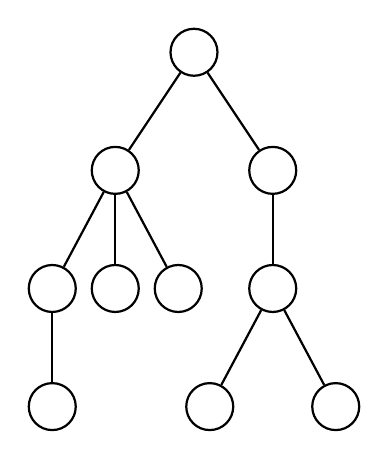
\begin{tikzpicture}[thick]
    \tikzset{node/.style={draw, circle, inner sep=6pt}};

    % Root
    \path (0, 0) coordinate [node] (r);

    % Level 1
    \path (-1, -1.5) coordinate [node] (l1a);
    \path (+1, -1.5) coordinate [node] (l1b);

    % Level 2
    \path (-1.8, -3) coordinate [node] (l2a);
    \path (-1, -3) coordinate [node] (l2b);
    \path (-0.2, -3) coordinate [node] (l2c);

    \path (+1, -3) coordinate [node] (l2d);

    % Level 3
    \path (-1.8, -4.5) coordinate [node] (l3a);

    \path (+0.2, -4.5) coordinate [node] (l3b);
    \path (+1.8, -4.5) coordinate [node] (l3c);

    % Edges
    \foreach \i in {a, b} { \draw (r) -- (l1\i); }
    \foreach \i/\j in {a/a, a/b, a/c, b/d} { \draw (l1\i) -- (l2\j); };
    \foreach \i/\j in {a/a, d/b, d/c} { \draw (l2\i) -- (l3\j); };
  \end{tikzpicture}

  \vspace{0.6cm}
  {\Large \textbf{AST}}
\end{slide}

% 1) Was ist ein AST actually?
% Ein AST heisst *abstrakt*, weil ein Knoten ueber ein abstraktes Interface
% dargestellt wird, zur Laufzeit aber Element aus einer Familie von konkreten
% Knotentypen ist. Selbes gilt fuer die Kinder des Knoten.
% Bei uns sind die moeglichen konkreten Typen:

\begin{slide}{Abstrakte Knoten}
  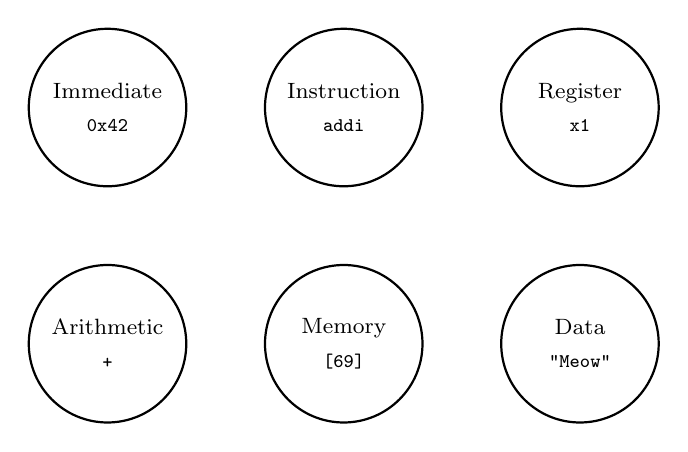
\begin{tikzpicture}[thick]
    \draw (0, 0) circle [radius=1cm] node [align=center]
          {\footnotesize Instruction\\ \scriptsize \texttt{addi}};

    \pause
    \draw (-3, 0) circle [radius=1cm] node [align=center]
          {\footnotesize Immediate\\ \scriptsize \texttt{0x42}};

    \pause
    \draw (+3, 0) circle [radius=1cm] node [align=center]
          {\footnotesize Register\\ \scriptsize \texttt{x1}};

    \pause
    \draw (-3, -3) circle [radius=1cm] node [align=center]
          {\footnotesize Arithmetic \\ \scriptsize \texttt{+}};

    \pause
    \draw (0, -3) circle [radius=1cm] node [align=center]
          {\footnotesize Memory \\ \scriptsize \texttt{[69]}};

    \pause
    \draw (+3, -3) circle [radius=1cm] node [align=center]
          {\footnotesize Data\\ \scriptsize \texttt{"Meow"}};
  \end{tikzpicture}

\end{slide}

\begin{slide}{Beispiel}
  \LARGE\texttt{add eax, [4*ebx+ecx+9]}
\end{slide}

\begin{slide}{Beispiel}
  \scalebox{0.7}{
  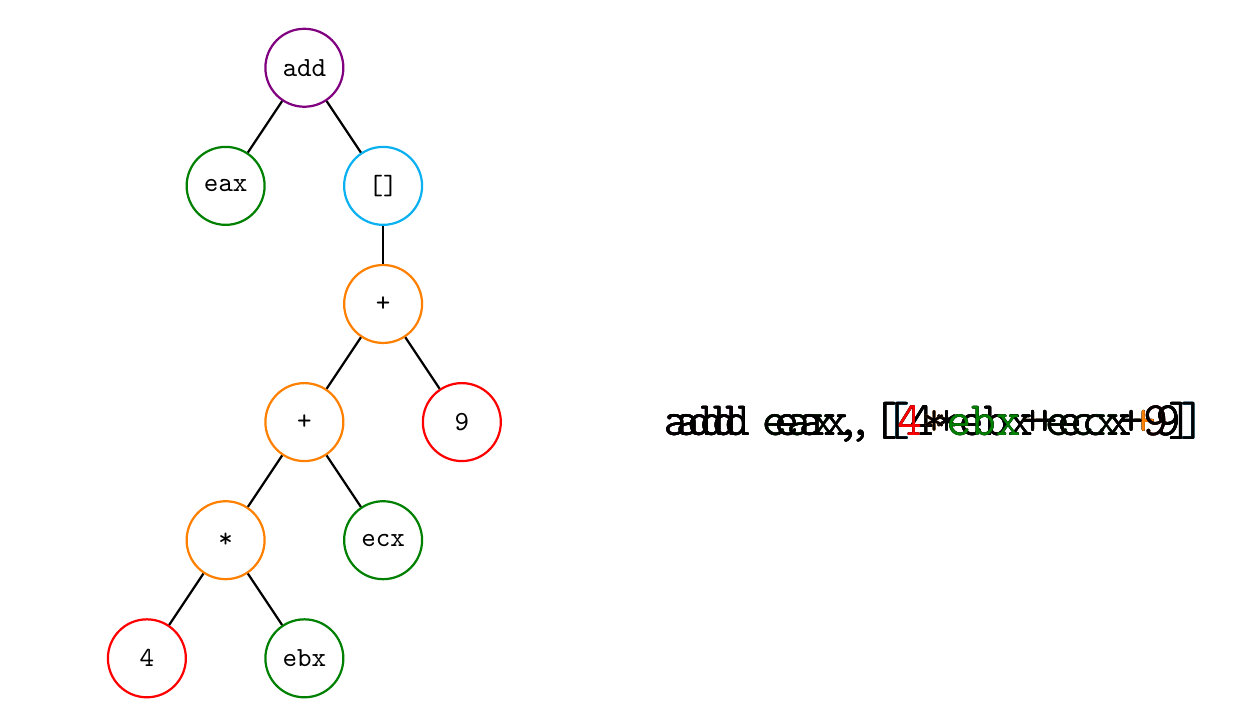
\begin{tikzpicture}[thick]
    \tikzset{node/.style={draw, circle, inner sep=0.35cm}};

    %%%%%%%%
    % Code %
    %%%%%%%%
    \onslide<1>{
      \node (code) at (8, -4.5) {\LARGE\texttt{add eax, [4*ebx+ecx+9]}};
    }
    \onslide<2>{
      \node (code) at (8, -4.5) {%
        \LARGE\texttt{\textcolor{Purple}{add} eax, [4*ebx+ecx+9]}
      };
    }
    \onslide<3>{
      \node (code) at (8, -4.5) {%
        \LARGE\texttt{add \textcolor{Green}{eax}, %
        \textcolor{ProcessBlue}{[}4*ebx+ecx+9\textcolor{ProcessBlue}{]}}
      };
    }
    \onslide<4>{
      \node (code) at (8, -4.5) {%
        \LARGE\texttt{add eax, [4*ebx+ecx\textcolor{orange}{+}9]}
      };
    }
    \onslide<5>{
      \node (code) at (8, -4.5) {%
        \LARGE\texttt{add eax,%
        [4*ebx\textcolor{orange}{+}ecx+\textcolor{Red}{9}]}
      };
    }
    \onslide<6>{
      \node (code) at (8, -4.5) {%
        \LARGE\texttt{add eax,%
        [4\textcolor{orange}{*}ebx+\textcolor{Green}{ecx}+9]}
      };
    }
    \onslide<7>{
      \node (code) at (8, -4.5) {%
        \LARGE\texttt{add eax,%
        [\textcolor{Red}{4}*\textcolor{Green}{ebx}+ecx+9]}};
    }

    % Left Spacer
    \draw (-3.5, 0);

    %%%%%%%%
    % Tree %
    %%%%%%%%

    % Root (instruction)
    \onslide<2->{
      \path (0, 0) coordinate [Purple, node] (add) node {\texttt{add}};
    }

    % Level 1 (eax, [])
    \onslide<3->{
      \path (-1, -1.5) coordinate [Green, node] (eax) node {\texttt{eax}};
      \path (+1, -1.5) coordinate [ProcessBlue, node] (mem) node {\texttt{[]}};

      \draw (add) -- (eax);
      \draw (add) -- (mem);
    }

    % Level 2 (plus)
    \onslide<4->{
      \path (+1, -3) coordinate [orange, node] (+1) node {\texttt{+}};
      \draw (mem) -- (+1);
    }

    % Level 3 (plus, 9)
    \onslide<5->{
      \path ( 0, -4.5) coordinate [orange, node] (+2) node {\texttt{+}};
      \path (+2, -4.5) coordinate [Red, node] (9) node {\texttt{9}};

      \draw (+1) -- (+2);
      \draw (+1) -- (9);
    }

    % Level 4 (*, ecx)
    \onslide<6->{
      \path (-1, -6) coordinate [orange, node] (*) node {\texttt{*}};
      \path (+1, -6) coordinate [Green, node] (ecx) node {\texttt{ecx}};

      \draw (+2) -- (*);
      \draw (+2) -- (ecx);
    }

    % Level 5 (6, ebx)
    \onslide<7->{
      \path (-2, -7.5) coordinate [Red, node] (4) node {\texttt{4}};
      \path ( 0, -7.5) coordinate [Green, node] (ebx) node {\texttt{ebx}};

      \draw (*) -- (4);
      \draw (*) -- (ebx);
    }
  \end{tikzpicture}
  }
\end{slide}
